\documentclass[aspectratio=169,11pt]{beamer}
\usetheme{NYUViolet}

\usepackage{array}
\usepackage{amsmath}
\usepackage{booktabs}
\usetikzlibrary{arrows.meta,backgrounds,calc,fit,positioning,shapes.geometric}

\graphicspath{{../Verilog-Adders/docs/diagrams/png/}}
\hypersetup{
  pdftitle={Adder Projects: Architecture, Generation, Verification, and Optimization},
  pdfauthor={Design Project I --- GenAI for Chip Design}
}

\title[Adder Projects]{Adder Projects}
\subtitle{Architecture, LLM-Based RTL Generation,\\Coverage-Driven Verification, and Yosys Optimization}
\author{Design Project I --- GenAI for Chip Design}
\date{Fall 2026}
\nyucourse{GenAI for Chip Design}
\setpartcount{3}

\tikzset{
  pflow/.style={nyubox,minimum width=2.55cm,minimum height=1.02cm,
    text width=2.35cm,font=\small},
  pflowtwo/.style={good,minimum width=2.55cm,minimum height=1.02cm,
    text width=2.35cm,font=\small},
  parr/.style={-{Stealth[length=2.2mm]},line width=.8pt,color=nyugray},
  pfeedback/.style={-{Stealth[length=2.1mm]},line width=.75pt,color=benign,dashed}
}

% The generated figures contain their own titles and generous margins. On
% lecture slides, crop those elements so the circuit itself remains legible.
\newcommand{\adderfigure}[1]{%
  \makebox[\linewidth][c]{%
    \includegraphics[width=1.05\linewidth,trim=4bp 42bp 4bp 52bp,clip]{#1}}}

\begin{document}

% ---------------------------------------------------------------------
\begin{frame}[plain,noframenumbering]
  \titlepage
\end{frame}

% ---------------------------------------------------------------------
\begin{frame}{In this presentation...}
  \begin{columns}[c,onlytextwidth]
    \column{0.45\textwidth}
      \small
      \begin{tikzpicture}[x=1cm,y=1cm]
        \foreach \n/\t [count=\i] in
          {1/{Project 1 \& Project 2},
           2/{Adder architectures},
           3/{Project 1 requirements}} {
          \node[nyuhead,minimum width=.72cm,minimum height=.72cm,font=\small\bfseries]
            (n\i) at (0,-1.25*\i) {\n};
          \node[anchor=west,font=\small,text width=4.7cm]
            at (.55,-1.25*\i) {\t};
        }
        \foreach \i/\j in {1/2,2/3}
          \draw[nyumist,line width=1.2pt] (n\i.south) -- (n\j.north);
      \end{tikzpicture}
    \column{0.51\textwidth}
      \begin{card}[fontupper=\footnotesize]{Goals}
        \begin{itemize}\setlength{\itemsep}{2pt}
          \item Connect Project 1 verification to Project 2 optimization
          \item Recognize six carry-computation strategies
          \item Identify what must survive an 8-to-16-bit scale-up
          \item Use the Project 1 PDF as the authoritative requirements document
        \end{itemize}
      \end{card}
  \end{columns}
  \vspace{-5pt}
  \takeaway{{\footnotesize Architecture connects generation, verification, and optimization.}}
\end{frame}

% =====================================================================
\section{Project 1 \& Project 2 Overview}
% =====================================================================

\begin{frame}{Two projects, one continuous design trajectory}
  \centering
  \resizebox{.95\textwidth}{!}{%
  \begin{tikzpicture}[node distance=.42cm]
    \node[pflow,font=\footnotesize] (study) {Study an existing\\8-bit architecture};
    \node[pflow,font=\footnotesize,right=of study] (spec) {Write a human-authored\\16-bit specification};
    \node[pflow,font=\footnotesize,right=of spec] (verify) {Generate, repair,\\cover, and verify RTL};
    \node[pflowtwo,font=\footnotesize,right=.72cm of verify] (opt) {Use Yosys feedback\\to optimize PPA};
    \draw[parr] (study) -- (spec);
    \draw[parr] (spec) -- (verify);
    \draw[parr] (verify) -- (opt);
    \node[draw=nyuviolet,dashed,rounded corners=4pt,fit=(study)(spec)(verify),inner sep=.22cm,
      label={[text=nyuviolet,font=\bfseries\small]below:Project 1}] {};
    \node[draw=benign,dashed,rounded corners=4pt,fit=(opt),inner sep=.22cm,
      label={[text=benign,font=\bfseries\small]below:Project 2}] {};
  \end{tikzpicture}}

  \vspace{.27cm}
  \begin{cardrow}{2}
    \begin{card}[fontupper=\footnotesize]{Project 1 establishes trust}
      \begin{itemize}\setlength{\itemsep}{1pt}
        \item Functional correctness
        \item Architectural fidelity
        \item Coverage quality and reproducibility
      \end{itemize}
    \end{card}
    \begin{goodcard}[fontupper=\footnotesize]{Project 2 searches for improvement}
      \begin{itemize}\setlength{\itemsep}{1pt}
        \item Area, delay, and balanced objectives
        \item Iterative LLM--Yosys feedback
        \item Equivalence and regression verification
      \end{itemize}
    \end{goodcard}
  \end{cardrow}
\end{frame}

\begin{frame}{Project 1: architecture-guided scaling and verification}
  \begin{columns}[T,onlytextwidth]
    \column{.57\textwidth}
      \small
      \begin{enumerate}
        \item \textbf{Understand} one existing 8-bit structural adder.
        \item \textbf{Specify} how that architecture becomes a 16-bit design.
        \item \textbf{Generate and repair} RTL using LLM output plus compiler feedback.
        \item \textbf{Generate stimulus} and refine it using coverage analysis.
        \item \textbf{Verify} with a Python golden model and self-checking testbench.
        \item \textbf{Compare} LLM-only tests with coverage-optimized tests.
      \end{enumerate}
    \column{.40\textwidth}
      \begin{card}[fontupper=\footnotesize]{Central requirement}
        The natural-language specification is a design artifact written from genuine RTL understanding.
      \end{card}
      \vspace{7pt}
      \begin{alertcard}[fontupper=\footnotesize]{Not acceptable}
        Replacing a required structural architecture with a one-line behavioral addition.
      \end{alertcard}
  \end{columns}
  \source{Project 1: Architecture-Guided Adder Scaling, RTL Generation, and Coverage-Driven Verification, Fall 2026.}
\end{frame}

\begin{frame}{Project 2: Yosys-guided PPA optimization}
  \begin{columns}[c,onlytextwidth]
    \column{.56\textwidth}
      \centering
      \begin{tikzpicture}[scale=.84,every node/.style={transform shape},node distance=.45cm and .65cm]
        \node[pflowtwo] (rtl) {Verified RTL\\and testbench};
        \node[pflowtwo,right=of rtl] (yosys) {Yosys synthesis\\and PPA report};
        \node[pflowtwo,below=of yosys] (feedback) {Metrics + failures\\returned to the LLM};
        \node[pflowtwo,left=of feedback] (candidate) {New architecture\\candidate};
        \draw[parr] (rtl) -- (yosys);
        \draw[pfeedback] (yosys) -- (feedback);
        \draw[pfeedback] (feedback) -- (candidate);
        \draw[pfeedback] (candidate) -- (rtl);
      \end{tikzpicture}
    \column{.41\textwidth}
      \begin{goodcard}[fontupper=\scriptsize]{Optimization modes}
        Area minimization, delay minimization, and balanced exploration.
      \end{goodcard}
      \vspace{5pt}
      \begin{card}[fontupper=\scriptsize]{Evidence}
        PPA trajectories, architecture explanations, synthesis logs, and best candidates.
      \end{card}
      \vspace{5pt}
      \begin{alertcard}[fontupper=\scriptsize]{Guardrail}
        Simulation and equivalence checking must confirm that optimization preserves function.
      \end{alertcard}
  \end{columns}
\end{frame}

\begin{frame}{Shared quality gates across both projects}
  \begin{cardrow}{2}
    \begin{card}{1 --- Function}
      Does every tested input produce the correct sum and carry?
    \end{card}
    \begin{card}{2 --- Architecture}
      Does the RTL preserve the assigned carry mechanism and hierarchy?
    \end{card}
    \begin{goodcard}{3 --- Verification}
      Did coverage expose untested structures and signal behaviors?
    \end{goodcard}
    \begin{goodcard}{4 --- Optimization}
      Are PPA gains reproducible and functionally safe?
    \end{goodcard}
  \end{cardrow}
  \takeaway{Generated output is untrusted until tools and human reasoning agree.}
\end{frame}

% =====================================================================
\section{Adder Architectures}
% =====================================================================

\begin{frame}{Architecture landscape}
  \footnotesize
  \begin{nyutable}{colspec={Q[wd=2.55cm] Q[wd=5.2cm] X},
      column{1}={font=\bfseries},rowsep=1pt}
    Architecture & Carry strategy & Main scaling question \\
    RCA & Serial full-adder chain & How many stages lie on the longest carry path? \\
    CLA & Expanded generate/propagate logic & How are higher-order carry equations organized? \\
    CSA & Compute both carry assumptions, then select & What group size and mux chain are used? \\
    Carry Skip & Ripple within blocks; bypass propagating blocks & Where are block boundaries and skip conditions? \\
    Kogge--Stone & Parallel-prefix tree & How many distance-doubling levels are required? \\
    Hybrid & Compose different carry structures & Where is the boundary, and how is carry handed off? \\
  \end{nyutable}
\end{frame}

\begin{frame}{Ripple Carry Adder (RCA)}
  \begin{columns}[c,onlytextwidth]
    \column{.70\textwidth}
      \adderfigure{ripple-carry.png}
    \column{.28\textwidth}
      \begin{card}[fontupper=\footnotesize]{What to preserve}
        \textbf{Carry idea:} each stage waits for the previous carry.\par\smallskip
        \textbf{Trade-off:} small and regular; delay grows linearly.\par\smallskip
        \textbf{8 $\rightarrow$ 16:} extend the full-adder chain and audit every carry connection.
      \end{card}
  \end{columns}
  \source{Course/FinalProjects/Verilog-Adders: RCA4.v and RCA8.v.}
\end{frame}

\begin{frame}{Carry Lookahead Adder (CLA)}
  \begin{columns}[c,onlytextwidth]
    \column{.70\textwidth}
      \adderfigure{carry-lookahead.png}
    \column{.28\textwidth}
      \begin{card}[fontupper=\footnotesize]{What to preserve}
        \textbf{Carry idea:} generate/propagate logic forms carries in parallel.\par\smallskip
        \textbf{Trade-off:} shorter latency; greater fan-in and equation complexity.\par\smallskip
        \textbf{8 $\rightarrow$ 16:} expand or hierarchically group carry equations without reintroducing ripple behavior.
      \end{card}
  \end{columns}
  \source{Course/FinalProjects/Verilog-Adders: CLA4.v and CLA8.v.}
\end{frame}

\begin{frame}{Carry Select Adder (CSA)}
  \begin{columns}[c,onlytextwidth]
    \column{.70\textwidth}
      \adderfigure{carry-select.png}
    \column{.28\textwidth}
      \begin{card}[fontupper=\footnotesize]{What to preserve}
        \textbf{Carry idea:} precompute candidates for carry-in 0 and 1, then select.\par\smallskip
        \textbf{Trade-off:} short selection path; duplicated arithmetic hardware.\par\smallskip
        \textbf{8 $\rightarrow$ 16:} define group sizes and connect each real carry to the correct mux controls.
      \end{card}
  \end{columns}
  \source{Course/FinalProjects/Verilog-Adders: CSA4.v and CSA8.v.}
\end{frame}

\begin{frame}{Carry Skip Adder (CSkipA)}
  \begin{columns}[c,onlytextwidth]
    \column{.70\textwidth}
      \adderfigure{carry-skip.png}
    \column{.28\textwidth}
      \begin{card}[fontupper=\footnotesize]{What to preserve}
        \textbf{Carry idea:} ripple inside a block; bypass it when every bit propagates.\par\smallskip
        \textbf{Trade-off:} moderate cost and faster long-distance carry movement.\par\smallskip
        \textbf{8 $\rightarrow$ 16:} preserve block boundaries, block-propagate equations, and mux polarity.
      \end{card}
  \end{columns}
  \source{Course/FinalProjects/Verilog-Adders: CSkipA4.v and CSkipA8.v.}
\end{frame}

\begin{frame}{Kogge--Stone Adder (KSA)}
  \begin{columns}[c,onlytextwidth]
    \column{.70\textwidth}
      \adderfigure{kogge-stone.png}
    \column{.28\textwidth}
      \begin{card}[fontupper=\footnotesize]{What to preserve}
        \textbf{Carry idea:} aligned Square, Big Circle, and Small Circle prefix operators.\par\smallskip
        \textbf{Trade-off:} logarithmic depth; high wiring density and node count.\par\smallskip
        \textbf{8 $\rightarrow$ 16:} add the distance-8 prefix level and verify every group boundary.
      \end{card}
  \end{columns}
  \source{Course/FinalProjects/Verilog-Adders: KSA4.v and KSA8.v.}
\end{frame}

\begin{frame}{Hybrid Adder (HA8)}
  \begin{columns}[c,onlytextwidth]
    \column{.70\textwidth}
      \adderfigure{hybrid.png}
    \column{.28\textwidth}
      \begin{card}[fontupper=\footnotesize]{What to preserve}
        \textbf{Carry idea:} combine architectures with an explicit carry handoff.\par\smallskip
        \textbf{Repository example:} CLA4 low half plus KSA4 high half.\par\smallskip
        \textbf{8 $\rightarrow$ 16:} state the new partition and preserve boundary-carry semantics.
      \end{card}
  \end{columns}
  \source{Course/FinalProjects/Verilog-Adders: HA8.v.}
\end{frame}

% =====================================================================
\section{Project 1 Requirements: Refer to the PDF}
% =====================================================================

\begin{frame}{The Project 1 PDF is the source of truth}
  \begin{columns}[c,onlytextwidth]
    \column{.40\textwidth}
      \centering
      \fcolorbox{nyurule}{white}{%
        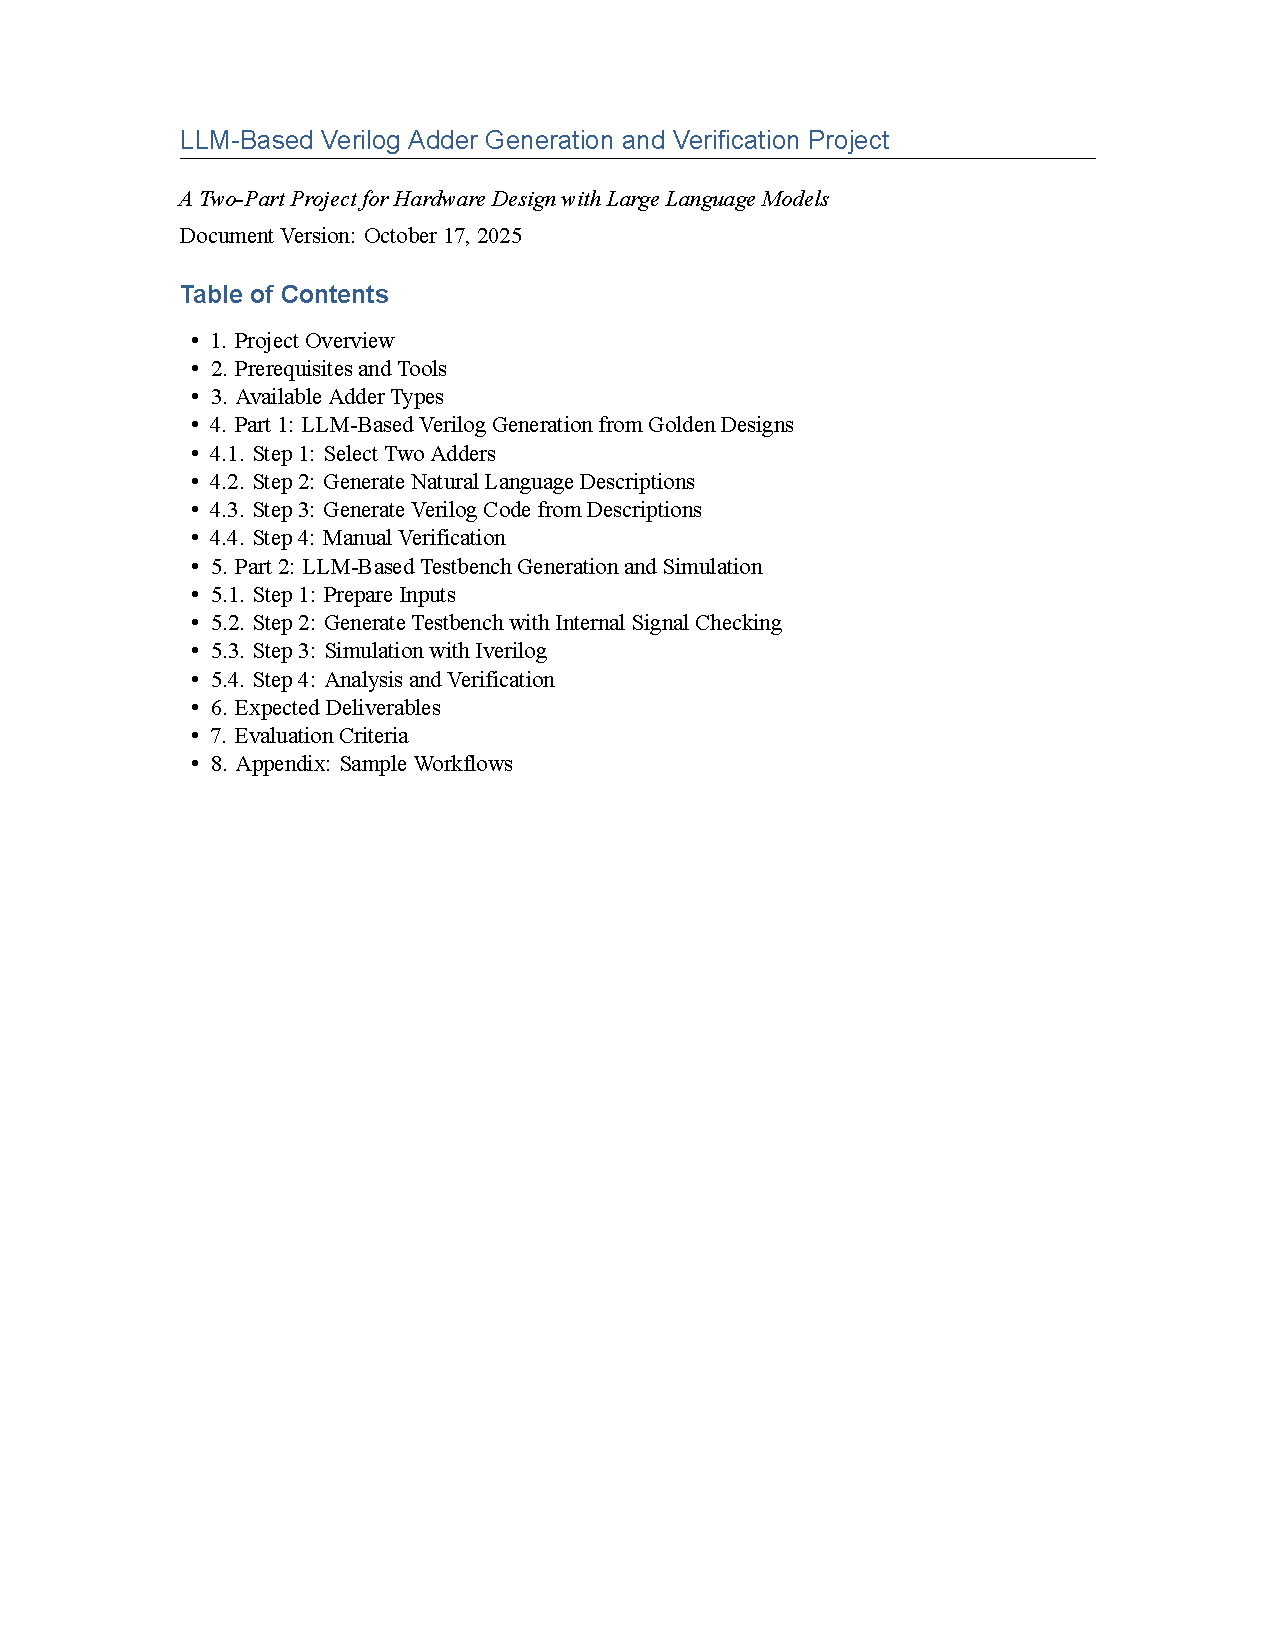
\includegraphics[page=1,height=.53\textheight]{../Verilog Adder Generation.pdf}}
    \column{.56\textwidth}
      \begin{card}[fontupper=\scriptsize]{Authoritative requirements document}
        \textbf{Project 1: Architecture-Guided Adder Scaling, RTL Generation, and Coverage-Driven Verification}\par\smallskip
        \texttt{Course/FinalProjects/}\par
        \texttt{Verilog Adder Generation.pdf}
        \begin{itemize}\setlength{\itemsep}{1pt}
          \item 13 pages, Fall 2026 version
          \item Authoritative phases, tools, coverage targets, deliverables, and evaluation criteria
          \item Architecture-specific questions and completion checklist
        \end{itemize}
      \end{card}
      \vspace{4pt}
      \begin{alertcard}[fontupper=\scriptsize]{In class}
        Walk through the PDF directly; if the slides and PDF differ, follow the PDF.
      \end{alertcard}
      \vspace{3pt}
      \href{run:../Verilog Adder Generation.pdf}{\beamergotobutton{Open the Project 1 PDF}}
  \end{columns}
\end{frame}

\begin{frame}{Before we open the PDF}
  \begin{cardrow}{2}
    \begin{card}{Keep these distinctions clear}
      \begin{itemize}\setlength{\itemsep}{3pt}
        \item Correct arithmetic vs. correct architecture
        \item Generated stimulus vs. self-checking verification
        \item Coverage evidence vs. correctness evidence
        \item Repairing RTL vs. refining tests
      \end{itemize}
    \end{card}
    \begin{goodcard}{Questions the PDF will answer}
      \begin{itemize}\setlength{\itemsep}{3pt}
        \item What exactly must be submitted?
        \item Which artifacts must be preserved?
        \item What coverage metrics and stopping conditions apply?
        \item How will the work be evaluated?
      \end{itemize}
    \end{goodcard}
  \end{cardrow}
  \takeaway{Now move to the Project 1 PDF.}
\end{frame}

% ---------------------------------------------------------------------
{\setbeamertemplate{footline}{}
\begin{frame}[plain,noframenumbering]
  \begin{tikzpicture}[remember picture,overlay]
    \fill[nyuviolet] (current page.south west) rectangle (current page.north east);
    \fill[white] ([xshift=.75cm,yshift=1.55cm]current page.west) rectangle ++(1.6cm,.1cm);
    \node[text=white,font=\fontsize{35}{38}\selectfont\bfseries,anchor=west]
      at ([xshift=.75cm,yshift=.5cm]current page.west) {Project 1 PDF};
    \node[text=nyumist,font=\small,anchor=north west,text width=10cm]
      at ([xshift=.75cm,yshift=-.35cm]current page.west)
      {Verilog Adder Generation.pdf \textbullet\ Source of truth for requirements};
  \end{tikzpicture}
\end{frame}}

\end{document}
